% Important: The shell-escape flag is required for the Minted package.
% Please compile this document with 'pdflatex -shell-escape main.tex'.
% If you are using another IDE, you may be able to specify this in the
% options or to provide an option like '% !TEX option = -shell-escape'
% in this file, depending on your builder. See the README.md for more.

% Don't put any content in here.
% Don't even include content files by using \input or \inlcude.
% Put your content into components/text.tex or include it there using \input.
% You probably want to modify the following files:
%   components/info.tex             contains the author, title etc.
%   components/settings.tex         contains the packages and settings.
%   components/commands.tex         contains helpful custom commands.
%   components/glossary.tex         contains an explanation of the used terms.
%   components/acknowledgements.tex contains the acknowledgements.
%   components/quote.tex            contains a quote.
%   components/abstract.tex         contains the abstract of the document.
%   components/text.tex             includes the actual content of the document.
%   components/outline.tex          contains the outline.
%   components/preface.tex          contains the preface.
%   chapters/                       contains the main text.
%   bibliography/literature.bib     contains the BibTeX entries.
%   images/                         contains all your content-related images.
%
% You probably don't need to change anything in the following files:
%   components/cover.tex            formats the front cover of the document.
%   components/titlepage.tex        formats the title page of the document.
%   components/disclaimer.tex       formats the disclaimer page.
%   styles/                         contains style elements (e.g. logos).
%   main.tex                        contains the top-level code structure.
%   README.md                       contains information about this template.

\documentclass[11pt,
              a4paper,
              tikz
              index=totoc,
              headsepline,
              footsepline,
              BCOR=12mm,
              DIV=13]{scrbook}

% KOMA scrbook options:
%  index=totoc: include an entry for the index in the table of contents.
%  headsepline: use horizontal line under heading.
%  footsepline: use horizontal line above footer.
%  BCOR: binding correction (e.g.: BCOR=12mm)
%  DIV: Number of sheet sections (used for layout) (e.g.: DIV=13)


%  This code base is currently hosted at: 
%  https://github.com/waltsims/TUM_Thesis_Template_CSE
             
% !TEX root = ../main.tex
% Set here the title, authors and other stuff to be used for the cover
% This file is used by MAIN.TEX

% set title, authors and stuff for the cover
\def\university{Technische Universit{\"a}t M{\"u}nchen}
\def\universityLogo{styles/tum_logo}
\def\program{Department of Informatics}
\def\programLogo{styles/faculty.pdf}
\def\doctype{Master's Thesis}

\def\title{Heterogeneous Quantum Computing with OPENQASM 3.0}
\def\author{Omar Ibrahim}
\def\examinerOne{Univ.-Prof.\ Dr.\ Christian Mendl}
\def\assistantAdvisor{Msc. Martin Knudsen}
\def\date{March 15th, 2023}

\def\keywords{{OPENQASM 3.0}, {Compiler}, {Heterogeneous Computing}}

% The following are used for the PDF metadata, by default the same as above.
\def\metaTitle{\title}
\def\metaAuthor{\author}
\def\metaSubject{\doctype\ -\ \university}
\def\metaKeywords{\keywords}

% text to appear in the footer
\def\footertext{}


% !TEX root = ../main.tex
% Included by MAIN.TEX

%--------------------------------------------------
% Fonts and page setup
%--------------------------------------------------

% Default font
\usepackage{palatino}

% \usepackage{listings}
% \lstset{language=C++}


% Enable special PostScript fonts (optional)
% \usepackage{pifont}

%use tikz for graphics

% Manipulate the footer
\usepackage{scrlayer-scrpage}
\usepackage{scrhack}
\pagestyle{scrheadings}
\ifoot[\footertext]{\footertext} % \footertext set in INFO.TEX

% Set the font for the section headings
\renewcommand{\sectfont}{\normalfont \bfseries}

% Conditional commands in LaTeX documents, used for the \clearemptydoublepage.
\usepackage{ifthen}

% Typeset text in multiple columns (optional)
% \usepackage{multicol}

% Rotation tools, including rotated full-page floats (optional)
\usepackage{rotating}



%--------------------------------------------------
% Document structure
%--------------------------------------------------

% Pro­duce hy­per­text links in the doc­u­ment (recommended)
\usepackage{hyperref}

% Create glossaries and lists of acronyms
% depending on how many packages were shipped with your TeX distribution,
% you might need to install xindy. On Linux: sudo apt install xindy
\usepackage[toc, xindy]{glossaries}

% Standard LaTeX package for creating indexes
\usepackage{makeidx}


%--------------------------------------------------
% Bibliography
%--------------------------------------------------

% Set the bibliography style (default: plain)
\bibliographystyle{plain}

% Special biblography package (nice to have)
% \usepackage{natbib}


%--------------------------------------------------
% Graphics and floats
%--------------------------------------------------

% Enhanced support for graphics (recommended)
\usepackage{graphicx}
% Path to the figures directory (default: {figures/})
% Multiple entries are allowed, e.g. {{figures1/}{figures2/}}.
\graphicspath{{figures/}}

% Improved interface for floating objects (optional)
\usepackage{float}

% To use the subfigures (optional)
\usepackage{subcaption}


%--------------------------------------------------
% Mathematics
%--------------------------------------------------

% AMS mathematical facilities for LaTeX (recommended)
\usepackage{amsmath}

% TeX fonts from the American Mathematical Society (recommended)
\usepackage{amsfonts}

% Some extra math symbols (optional)
% \usepackage{amssymb}

% Extended maths fonts for LaTeX (optional)
% \usepackage{yhmath}

% Provide math delimiters whose size can be computed automatically (optional)
% \usepackage{commath}


%--------------------------------------------------
% Source code and algorithms
%--------------------------------------------------

% Source code typesetting
% \usepackage{listings} % (optional - alternative)
\usepackage[newfloat]{minted} % (recommended)
% Set global Minted options
\setminted{linenos, autogobble, frame=lines, framesep=2mm}
% Inline C++ (optional)
\newcommand{\incpp}[1]{\mintinline{c++}{#1}}
\newenvironment{code}{\captionsetup{type=listing}}{}
\SetupFloatingEnvironment{listing}{name=Source Code}

% Typeset algorithms - pseudocode (optional)
% \usepackage{algorithmicx}
% \usepackage{algpseudocode}
% Normal arrow comments
% \algrenewcommand{\algorithmiccomment}[1]{\hfill$\rightarrow$ #1}


%--------------------------------------------------
% Tables
%--------------------------------------------------

% Tables (optional)
\usepackage{tabu}

% Add color to LaTeX tables (optional)
% \usepackage{colortbl}

% Create tabular cells spanning multiple rows (optional)
% \usepackage{multirow}


%--------------------------------------------------
% Color
%--------------------------------------------------

% Use colors
\usepackage[dvipsnames]{xcolor}

\usepackage{tikz}

\usepackage{svg}


% You may find all the pre-defined colors in
% https://en.wikibooks.org/wiki/LaTeX/Colors#Predefined_colors

% Custom colors
\definecolor{Pantone300C}{HTML}{0065BD} % TUM primary blue
\definecolor{Pantone301}{HTML}{005293}  % TUM secondary light blue
\definecolor{Pantone540}{HTML}{003359}  % TUM secondary dark blue
\definecolor{DarkGray}{HTML}{333333}    % TUM secondary dark gray
\definecolor{MediumGray}{HTML}{808080}  % TUM secondary medium gray
\definecolor{LightGray}{HTML}{CCCCC6}   % TUM secondary light gray
\definecolor{Pantone7527}{HTML}{DAD7CB} % TUM accent gray
\definecolor{Pantone158}{HTML}{E37222}  % TUM accent orange
\definecolor{Pantone383}{HTML}{A2AD00}  % TUM accent green
\definecolor{Pantone283}{HTML}{98C6EA}  % TUM accent very light blue
\definecolor{Pantone542}{HTML}{64A0C8}  % TUM accent light blue

% Color for the hyperlinks (e.g. table of contents)
\def\colorLinks{Pantone300C}
% Color for the web links
\def\colorUrl{Pantone542}
% Color for the citations
\def\colorCitations{Pantone158}

%--------------------------------------------------
% PDF output
%--------------------------------------------------

% Adjust the color of the links
\hypersetup{
  linkcolor=\colorLinks,%
  urlcolor=\colorUrl,%
  citecolor=\colorCitations
}

% Disable the coloring of the links when printing.
% Requires a compatible PDF reader.
\usepackage[ocgcolorlinks]{ocgx2}[2017/03/30]

% PDF Metadata
\hypersetup{
  pdftitle={\metaTitle},%
  pdfauthor={\metaAuthor},%
  pdfkeywords={\metaKeywords},%
  pdfsubject={\metaSubject}
}

% Create XMP Metadata (uses the values from hyperref)
\usepackage{hyperxmp}

% Make thumbnails (optional)
% \usepackage{thumbpdf}


%--------------------------------------------------
% Other settings
%--------------------------------------------------

% Define commands that appear not to eat spaces (optional)
\usepackage{xspace}


% !TEX root = ../main.tex
% Included by MAIN.TEX
% Please include your own cool commands here.
% Be only sure to comment it sufficiently so others can use it.

%-------------------------------------------------------------
%                      Own Commands
%-------------------------------------------------------------


%-------------------------------------------------------------
% math stuff -------------------------------------------------

% nice R, N, C
\newcommand{\nat}{\mathbb{N}}
\newcommand{\real}{\mathbb{R}}
\newcommand{\compl}{\mathbb{C}}

% un demi
\newcommand{\half}{\frac{1}{2}}

% parantheses
\newcommand{\parenth}[1]{ \left(#1 \right) }
\newcommand{\bracket}[1]{ \left[#1 \right] }
\newcommand{\accolade}[1]{ \left\{ #1 \right\} }
%\newcommand{\angle}[1]{ \left\langle  #1 \right\rangle }

% partial derivative: %#1 function, #2 which variable
% simple / single line version
\newcommand{\pardevS}[2]{ \delta_{#1} f(#2) }

% fraction version
\newcommand{\pardevF}[2]{ \frac{\partial #1}{\partial #2} }

% render vectors: 3 and 4 dimensional
\newcommand{\veciii}[3]{\left[ \begin{array}[h]{c} #1 \\ #2 \\ #3	\end{array} \right]}
\newcommand{\veciv}[4]{\left[ \begin{array}[h]{c} #1 \\ #2 \\ #3 \\ #4	\end{array} \right]}

% render matrices: 3  dimensional (arguments in row first order)
\newcommand{\matiii}[9]{\left[ \begin{array}[h]{ccc} #1 & #2 & #3 \\ #4 & #5 & #6 \\ #7 & #8 & #9	\end{array} \right]}

%-------------------------------------------------------------
% some abreviations ------------------------------------------
\newcommand{\Reg}{$^{\textregistered}$}
\newcommand{\reg}{$^{\textregistered}$ }
\newcommand{\Tm}{\texttrademark}
\newcommand{\tm}{\texttrademark~}
\newcommand {\bsl} {$\backslash$}

%-------------------------------------------------------------
% formating --------------------------------------------------

% Theorem & Co environments and counters
\newtheorem{theorem}{Theorem}[chapter]
\newtheorem{lemma}[theorem]{Lemma}
\newtheorem{corollary}[theorem]{Corollary}
\newtheorem{remark}[theorem]{Remark}
\newtheorem{definition}[theorem]{Definition}
\newtheorem{equat}[theorem]{Equation}
\newtheorem{example}[theorem]{Example}
%\newtheorem{algorithm}[theorem]{Algorithm}

% inserting figures
\newcommand{\insertfigure}[4]{ % Filename, Caption, Label, Width percent of textwidth
	\begin{figure}[htbp]
		\begin{center}
			\includegraphics[width=#4\textwidth]{#1}
		\end{center}
		\vspace{-0.4cm}
		\caption{#2}
		\label{#3}
	\end{figure}
}

% referecing figures

\newcommand{\refFigure}[1]{ %label
	Figure~\ref{#1}
}
\newcommand{\refChapter}[1]{ %label
	Chapter~\ref{#1}
}

\newcommand{\refSection}[1]{ %label
	Section~\ref{#1}
}

\newcommand{\refParagraph}[1]{ %label
	Paragraph~\ref{#1}
}

\newcommand{\refEquation}[1]{ %label
	Equation~\ref{#1}
}

\newcommand{\refTable}[1]{ %label
	Table~\ref{#1}
}

\newcommand{\rigidTransform}[2]
{
	${}^{#2}\!\mathbf{H}_{#1}$
}

% comment that appears on the border - very practical !!!
\newcommand{\comment}[1]{\marginpar{\raggedright \noindent \footnotesize {\textsl{#1}} }}

% page clearing
\newcommand{\clearemptydoublepage}{%
  \ifthenelse{\boolean{@twoside}}{\newpage{\pagestyle{empty}\cleardoublepage}}%
  {\clearpage}}

%-------------------------------------------------------------
%-------------------------------------------------------------

\newcommand{\etAl}{\emph{et al.}\mbox{ }}


% !TEX root = ../main.tex
\newglossaryentry{computer}
{
  name=computer,
  description={is a programmable machine that receives input,
               stores and manipulates data, and provides
               output in a useful format}
}

\newglossaryentry{poc}
{
  name={proof of concept},
  description={}
  }
\newglossaryentry{ui}
{
  name={user interface},
  description={}
  }
\newglossaryentry{ai}
{
  name={arithmetic intensity},
  description={a measure of floating-point operations (FLOPs)
              \hyphenation{per-formed} performed by a \hyphenation{gi-ven} given code or code section relative
              to the amount of memory accesses (Bytes) that are required
               to support those operations\cite{AI}}
  }

\newglossaryentry{speed-up}
{
  name={speed-up},
  description={the factor of temporal acceleration a program
  exhibits when additional computational resources are dedicated to it's execution.}
}

\newglossaryentry{directive pragmas}
{
  name={directive pragma},
  description={a computer programming language construct that specifies how a compiler
  should process input data} % sourced from wikipedia
}


\newglossaryentry{rc}{%SOURCE: wikipedia
name={race condition},
description={A race condition or race hazard is the behavior of an electronic,
 software, or other system where the output is dependent on the sequence or
 timing of other uncontrollable events. It becomes a bug when events do not
 happen in the order the programmer intended. The term originates with the idea
 of two signals racing each other to influence the output first.}
}
\newglossaryentry{dd}{
name={data dependencies},
description={}
}
\newglossaryentry{sisd}{
name={single instruction single data},
description={}
}
\newglossaryentry{simt}{
name={single instruction multiple threads},
description={}
}

\newglossaryentry{simd}{
name={single instruction multiple data},
description={}
}
\newglossaryentry{gp}{%SOURCE: wikipedia
name={Gaussian Plane},
description={The two dimensional plane of complex numbers.}
}
\newglossaryentry{CURAND}{
name={CURAND},
description={
The CURAND library provides facilities that focus on the simple and efficient
generation of high-quality pseudorandom and quasirandom numbers.\cite{cuRAND}
}
}

\newacronym[longplural={partial differential equations}]{PDE}{PDE}{partial differential equations}
\newacronym{mpi}{MPI}{Message Passing Interface}

\newacronym[longplural={Random Walks on Spheres}]{RWoS}{RWoS}{Random Walk on Spheres}

\newacronym[longplural={graphical processing units}]{GPU}{GPU}{graphical processing unit}

\newacronym[longplural={central processing units}]{CPU}{CPU}{central processing unit}
\newacronym{hpc}{HPC}{high performance computing}

\newacronym[longplural={arithmetic logic units}]{ALU}{ALU}{arithmetic logic unit}

\newacronym[longplural={streaming multi-processors}]{SM}{SM}{streaming multi-processor}

\newacronym[longplural={boundary value problems}]{BVP}{BVP}{boundary value problem}
\newacronym[longplural={general purpose graphical processing units}]{GPGPU}{GPGPU}{general purpose graphical processing units}
\newacronym{CUDA}{CUDA}{compute unified device architecture}
\newacronym{RAM}{RAM}{random access memory}
\newacronym{SRAM}{SRAM}{static random access memory}
\newacronym{DRAM}{DRAM}{dynamic random access memory}
\newacronym{I/O}{I/O}{input/output}
\newacronym{PTX}{PTX}{Parallel Thread eXecution}
\newacronym{jit}{JIT}{just in time}


\makeglossaries

\begin{document}

 \frontmatter

 % !TEX root = ../main.tex
% The front cover.
% Included by MAIN.TEX

%--------------------------------------------------
% The Front Cover
%--------------------------------------------------

% correct BCOR - undo at the end !!!
\def\bcorcor{0.15cm}
\addtolength{\hoffset}{\bcorcor}

\thispagestyle{empty}

\vspace{4cm}
\begin{center}
	\includegraphics[width=4cm]{\universityLogo}\\
	\vspace{5mm}
	\huge \program \\
	\vspace{0.5cm}
	\large \university
\end{center}

\vspace{20mm}
\begin{center}
	{\Large \doctype}\\
	\vspace{20mm}
	{\huge \textbf \title}\\
	\vspace{15mm}
	{\LARGE  \author}\\
	\vspace{\fill}
	\includegraphics[width=4cm]{\programLogo}
\end{center}


 \clearemptydoublepage

 % !TEX root = ../main.tex
% The titlepage.
% Included by MAIN.TEX


%--------------------------------------------------
% The title page
%--------------------------------------------------

% correct BCOR - undo at the end !!!
\def\bcorcor{0.15cm}
\addtolength{\hoffset}{\bcorcor}

\thispagestyle{empty}

\vspace{4cm}
\begin{center}
    \includegraphics[width=4cm]{\universityLogo}\\
    \vspace{5mm}
    \huge \program \\
    \vspace{0.5cm}
    \large \university
\end{center}

\vspace{10mm}
\begin{center}
    {\Large \doctype}\\
    \vspace{10mm}
    {\LARGE \title}\\
    \vspace{10mm}

    \begin{tabular}{ll}
      \Large Author:                        & \Large \author \\[2mm]
      \Large 1\textsuperscript{st} examiner:& \Large \examinerOne\\[2mm]
      \Large Assistant advisor:             & \Large \assistantAdvisor \\[2mm]
      \Large Submission Date:               & \Large \date
    \end{tabular}

    \vspace{\fill}
    \includegraphics[width=4cm]{\programLogo}
\end{center}

% undo BCOR correction
\addtolength{\hoffset}{\bcorcor}


 % !TEX root = ../main.tex
\clearemptydoublepage

\thispagestyle{empty}
\vspace*{0.8\textheight}
\noindent
I hereby declare that this thesis is entirely the result of my own work except where otherwise indicated. I have only used the resources given in the list of references.

\vspace{15mm}
\noindent
\date \hspace{5cm} \author
\newpage


 % !TEX root = ../main.tex
\clearemptydoublepage
\phantomsection
\addcontentsline{toc}{chapter}{Acknowledgements}

\vspace*{2cm}

\begin{center}
{\Large \textbf{Acknowledgments}}
\end{center}

\vspace{1cm}

\begin{center}
If someone helped you or supported you through your studies, this page is a
good place to tell them how thankful you are.
\end{center}


 \clearpage
\phantomsection

\begin{center}
\vspace*{11cm}
\textit{``Everything should be made as simple as possible. \\ But to do that you have to master complexity.''}
\end{center}
\par
\hspace*{7cm}
\textit{-Butler Lampson}


 % !TEX root = ../main.tex
% The abstract.
% Included by MAIN.TEX
\clearemptydoublepage
\phantomsection
\addcontentsline{toc}{chapter}{Abstract}

\vspace*{2cm}
\begin{center}
{\Large \textbf{Abstract}}
\end{center}
\vspace{1cm}

This document will serve as an example to you, of how to use \LaTeX to write your
CSE Master's Thesis. It will have examples and recomendations, and hopefully a
few laughs.  Because this is the abstract, it will have to convince you that this 
template is something you want to use.  It has been proven, that without using
this template, writing your thesis will be much more dificult. The template is
based on previous work, and has been improved apon and updated.  The result of 
this template is a modern latex template that everyone can contribute to and use
for their studies of CSE @ TUM.

Some more great abstract tips can be found here: 
\href{https://users.ece.cmu.edu/~koopman/essays/abstract.html}{Great Abstract tips}


 \tableofcontents

 \mainmatter

 % !TEX root = ../main.tex
% Included by MAIN.TEX
% Put your content in here or include it by using \input (\include won't work)

\addtolength{\evensidemargin}{-12mm}

% ---------------------------------------------------------------------------
%
%Introduction and Background Theory
%
% ---------------------------------------------------------------------------
\label{part:introduction}
% !TEX root = ../main.tex
\chapter{Introduction}
\label{chapter:Introduction}
Combination of quantum and classical computation as a form of Hetorgenous Computing allows us
to solve very interesting problems. Many quantum algorithms and applications relies
deeply on this combination. Whether near-time heterogenous computing (i.e: Variational Quantum Eigen Solver),
or real-time (i.e: quantum error correction algorithms). While near-time heterogenous computing
is already achievable with current technology, albeit on a small scale, 
real-time heterogenous computing is still a
challenge,
%TODO: fact check
due to the issue of decoherence time of quantum systems, and the requirement for
very low classical data transfer latency to account for this issue. In either
of these cases, we can use a quantum processing unit (QPU) as an accelerator
alongside a cpu, where the QPU can solve problems that QPU's excel in and the
CPU can solve problems that CPU's excel in, such as conditionals, loops...etc.
This allows us to apply quantum algorithms that uses a cpu as a co-processor,
but also to improve the performance of a a QPU as in the case of quantum error
correction.  This concept of heterogenousity can also be extended to include
other types of accelerators such as GPUs, FPGAs, and ASICs, to benefit from them
in domains where they excel. However, in this thesis we will focus on the
combination of quantum and classical computing. In this thesis we provide a compilation 
framework for OPENQASM 3.0, a quantum programming language that supports many classical instructions,
allowing for heterogenous computing. Previous workflows have been provided by this,
notably the QCOR framework, which was a great inspiration for this work. QCOR, and after that this work,
created dialects for lowering of OPENQASM 3.0 to MLIR, apply optimizations and then
execute this intermeidate representation on a QPU paired with a classical accelarator, or just execute it 
on a quantum simulator.
%maybe cite qcor?
In this work we approach this problem similarly, in a couple of aspects, moreover,
we noticed that the work on QCOR was discountinued, and the OPENQASM 3.0 spec was changing
frequently, and we wanted to keep up with the latest changes. 
% TODO: double check if we actually abide to the latest syntax,
% if not just mention that we tried to adhere to the latest available spec.
The difference in our approach are the following:
1- adhere to latest spec as of time of development
2- use latest MLIR version
3- make use of dialects such as the vector dialect, to allow for vectorization of 
operations and perform the much needed speed up of classical operations.
4- Provide an explicit lowering step to restricted gate sate matching quantum gates
available on desired hardware.
5- We did this step as a proof of concept of the possibility to lower a generic quantum dialect
to a restricted quantum dialect that has a specific set of quantum gates. We used quantum gates
supported by the Walter Meiner Institute(WMI)'s quantum computers, as an example.
6- Due to limitations faced by the quantum computing team in WMI, we were not able to execute
the quantum heterogenous generated MLIR code on their hardware.
However, as also another proof of conept, we created a quantum simulator written purely in MLIR
to test out our compilation pipeline, and to showcase the possiblity to write a quantum simulator purely in MLIR,
which could have superior perfromance to call external c++(or other languages) from within our MLIR code.

In the next section we provide a background about the differente topics for this thesis. 
FOllowed by the body were we showcase our approach to this
compilation pipeline, the key components in our codebase, the openqasm operation we 
supported, not all operations were supported but the set of operations can be extended. We also showcase
some example mlir code that was generated at 
different stages of our compilation pipeline.
Finally we show some basic quantum optimization that
we constructed using MLIR's pattern rewriter as part of the compilation passes,
as well as builtin mlir classical optimizations.
Finally, in the last chapeter we showcase our quantum
simulation and present some closing remarks about our works
and the future work that can extend the current one.

% This document has been created in order to show you some of the capabilities 
% of \LaTeX.  A great resource for an introduction to \LaTeX\xspace is Tobias
% Oetiker's ''The Not So Short Introduction to \LaTeXe'' \cite{latex}.  Please
% page through that document
% before starting with your thesis.
% Oh, and let's use the mysterious word \gls{computer} here to give the glossary
% a reason to appear.
% A third useful option to reference stuff besides citing or glossarying (?) 
% is using footnotes. Just like
% this\footnote{Properly formatted clickable URL: \url{https://www.tum.de/}}
% one.
% And: lists! Lists with bullet points are amazing. I mean, just look at this:
% \begin{itemize}
% 	\item list
% 	\item all 
% 	\item the 
% 	\item things!
% \end{itemize}
% % use enumerate for numbers instead of points: 
% % https://en.wikibooks.org/wiki/LaTeX/List_Structures#List_structures
% \par
% Anyways your introduction goes here.


% Below a few \LaTeX examples are included for beginners
% \comment{You can also put comments in the margins for you or your advisor}
% \begin{figure}[ht]
%   \centering
%   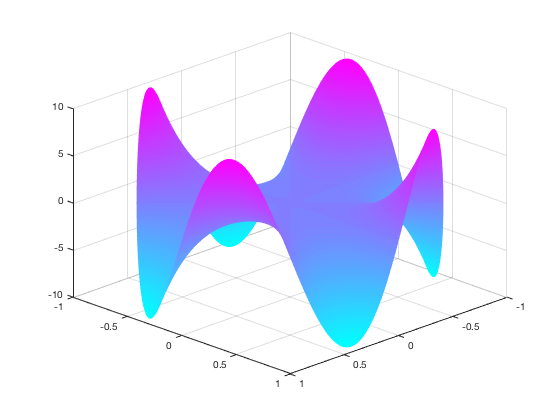
\includegraphics[width=5cm]{images/swing_function_plot.png}
%   \caption{$u(x)$}%{Numerically solved solution}
%   \label{fig:swingPlot}
% \end{figure}


% Equations can also be labeled
% \begin{equation}
% 	\pi = \mathrm{e}^{i\cdot\phi}
% 	\label{eq:equation1}
% \end{equation}


% And later referenced. Even in subfigures.
% \begin{figure}[!htb]
%   \centering
%   \begin{subfigure}[b]{0.3\textwidth}
%     \centering
%   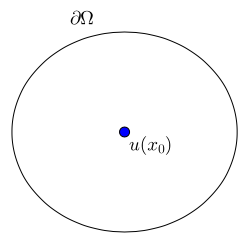
\includegraphics[width=\textwidth]{images/CircCenter}
%   \caption{Equation~\ref{eq:equation1}}\label{fig:circcenter}
% \end{subfigure}
% \hfill
%   \begin{subfigure}[b]{0.3\textwidth}
%     \centering
%   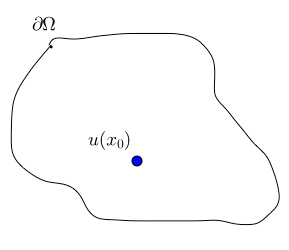
\includegraphics[width=\textwidth]{images/GeneralOffset}
%   \label{fig:generaloffset}
%   \caption{Equation~\ref{eq:equation1}}
% \end{subfigure}
% \end{figure}
% \section{Including code}

% Code can be using the package
% \href{https://www.sharelatex.com/learn/Code\_Highlighting\_with\_minted}{Minted}.

% An exaple of which of can be found below (see Source Code~\ref{lst:nice_listing})
% \begin{listing}
% 	%the language syntax can be declared here.
% 	\begin{minted}{python} 
% 	import numpy as np
	
% 	def incmatrix(genl1,genl2):
% 	    m = len(genl1)
% 	    n = len(genl2)
% 	    M = None #to become the incidence matrix
% 	    VT = np.zeros((n*m,1), int)  #dummy variable
	
% 	    #compute the bitwise xor matrix
% 	    M1 = bitxormatrix(genl1)
% 	    M2 = np.triu(bitxormatrix(genl2),1)
	
% 	    for i in range(m-1):
% 	        for j in range(i+1, m):
% 	            [r,c] = np.where(M2 == M1[i,j])
% 	            for k in range(len(r)):
% 	                VT[(i)*n + r[k]] = 1;
% 	                VT[(i)*n + c[k]] = 1;
% 	                VT[(j)*n + r[k]] = 1;
% 	                VT[(j)*n + c[k]] = 1;
	
% 	                if M is None:
% 	                    M = np.copy(VT)
% 	                else:
% 	                    M = np.concatenate((M, VT), 1)
	
% 	                VT = np.zeros((n*m,1), int)
	
% 	    return M
% 	\end{minted}

%   \caption{My nice listing}
%   \label{lst:nice_listing}
% \end{listing}

\chapter{Background}
% add figures
\label{chapter:Background}
\section{Heterogeneous Computing}
Heterogeneous computing refers to the use of multiple types of processing units
or cores within a single computer system. These processing units can include
central processing units (CPUs), graphical processing units (GPUs), 
field programmable hate arrays (FPGAs), and application-specific integrated circuits(ASICs), each of which can perform
specific types of computations with varying degrees of efficiency. The goal of
heterogeneous computing is to leverage the strengths of each processing unit to
improve the overall performance and energy efficiency of the system. For our
purposes we will focus on heterogeneous computing that combines classical
computing using CPUs and quantum computing using quantum processing units (QPUs), quantum-classical
heterogeneous computing.
In this kind of heterogeneous computing we face the challenge of quantum
decoherence. Quantum decoherence is the phenomenon where quantum systems interact
with the environment, causing them to lose their
quantum behavior and fallback to a classical one.
These two challenges are different depending on whether we are applying
near-time or real-time quantum computing. Real-time quantum computing requires calculations to
complete within - or faster than - the qubit coherence time, while near-time quantum computing can tolerate high
latency.
% paraphrase
\section{Quantum Computing Programming}
Quantum computing programming languages are designed to help developers write
and execute quantum algorithms on quantum computers. Although quantum computers
are still in the early stages of development, there has been significant
progress in the development of quantum computing programming languages. In this
thesis we are only interested in OPENQASM 3.0. OPENQASM - short for Open Quantum
Assembly - is a low level, quantum circuit-like language for quantum computing.
With its newest edition - OPENQASM 3.0 - OPENQASM is no longer a strictly
quantum programming language, but rather a Heterogeneous language. It allows for
strictly quantum operations provided in OPENQASM 2.0, but also allows classical
operations such as control operations (i.e: for and while loops, if
statements...etc), extensive arithmetic operations, among many other operations.
This heterogeneity of the language, being an open standard, and the large
adoption by many scientists are all reasons for focusing on OPENQASM 3.0 in this
thesis.
\section{Compilation}
\subsection{Compilation Overview}
Compilation in computer science is the process of translating a source language
to a target language. Typically, this is done in an effort to translate a
high-level language, to a lower level language, or to machine code to be executed by
the computer. Normally, a compiler has two main parts, the frontend and the backend.
The frontend applies the analysis phase of a compiler, while the backend applies
the synthesis phase. The analysis phase, among possibly other steps, has three
main steps:
\begin{itemize}
  \item Lexical Analysis
  \item Syntax Analysis
  \item Semantic Analysis
\end{itemize}
Lexical analysis, also called tokenization, is the process of splitting the
input file into multiple tokens. If invalid tokens are found a tokenization
error is generated. Syntax analysis, also known as parsing, is the process of
verifying that a token stream is syntactically well-formed, and constructs a
syntax tree from a valid set of tokens. This essentially verifies that the input program
abides to our language's grammar syntax, and provides an intermediate
representation for the next stage of analysis. The program that performs the
parsing is called the parser. Finally, semantic analysis is the process of
verifying that our program is sound in regard to our language's semantics. For
example, in a strictly typed language an int variable can't be assigned a
string. During semantic analysis, the syntax tree can be annotated to provide
useful information (i.e: implicit type casting information) and produces what is
known as an abstract syntax tree.

The next stage, the synthesis phase, consists also of three main phases:
\begin{itemize}
  \item Intermediate Code Generation
  \item Program Optimization
  \item Code Generator
\end{itemize}
Intermediate code generation is the process of generating a low-level
intermediate representation (IR) code. This IR usually has the benefit of having
a small instruction set, and simple syntax and semantics. This makes the next stage, 
the program optimization stage, much simpler.
Program optimization is the process of transformation from a less efficient program 
to a more efficient one. This can be done by removing redundant instructions,
or instructions with more efficient ones. Intuitively, this stage is optional yet
very essential. It can be split into two stages, machine independent and machine
dependent optimization, where the former is done before target code generation,
and the latter is done after.
Finally, target code generation is the process of generating the
target code to be executed on the machine. %TODO: makes this more concise
\subsection{ANTLR}
ANTLR (Another Tool for Language Recognition) is a parser generator that can
read, analyze, execute, or translate structured text or binary files. It's often
used in the creation of programming languages, tools, and frameworks
\cite{ANTLR}. ANTLR generates a parser from a grammar defined in a domain
specific language (DSL), designed by ANTLR. ANTLR provides runtimes in multiple
programming languages. You can choose which runtime you want your parser to be
written in, and then you can construct and walk parse trees from input programs.
\subsection{LLVM and MLIR}
\subsubsection{LLVM}
LLVM, which stands for Low Level Virtual Machine, is a compiler framework that
enables comprehensive program analysis and transformation for various programs
throughout their entire lifespan. It does this by providing high-level
information to compiler transformations at compile-time, link-time, run-time,
and in idle time between runs. LLVM uses a common, low-level code representation
in Static Single Assignment (SSA) form, which includes a simple,
language-independent type-system that exposes the primitives commonly used to
implement high-level language features. Additionally, LLVM features an
instruction for typed address arithmetic and a simple mechanism that can be used
to implement the exception handling features of high-level languages and
\texttt{setjmp}/\texttt{longjmp} in C uniformly and efficiently.
\subsection{MLIR}
Multi-level intermediate representation (MLIR) is a novel approach for creating
reusable and adaptable domain specific compilers. It is designed to provide an
extensible common IR of SSA form, that can be used to represent multiple Domain
specific languages (DSLs). This elevates the need for a new IR for each new DSL
language, and allows for the reuse of existing IRs, especially within the same
domain. Moreover, MLIR can be then lowered to LLVM IR, and utilize the LLVM
tool-chain providing multiple lower-level optimizations and the ability to target
different kinds of hardware accelerators with different architectures. The
structure of MLIR's IR has few key abstractions - types, attributes, and
operations. These main three abstractions can sufficiently extend the IR to its
users needs. There are two more abstractions, regions and blocks, but they are
extension of operations, where a block is a list of operations, and a region is
a list of blocks. A Dialect refers to a unique namespace that encompasses a
coherent set of operations, types, and attributes that are logically grouped
together. MLIR provides a lot of public dialects catering to different domains,
such as the Arith Dialect, the Math Dialect, the \texttt{MemRef} (Memory Reference) Dialect,
and the Vector Dialect...etc. One can also create their own dialect 
for their own domain specific application. MLIR also provides a set of tools to
help with the creation of new dialects, such as the MLIR \texttt{TableGen} tool, which
allows for the creation of new dialects by writing a simple DSL.
However, it should be noted that if one desires to lower down to LLVM IR, they
will have to lower their dialect's operations in terms of the dialects provided 
by MLIR (include the LLVM IR). There are multiple approaches and defined classes that can aid with that.
\subsection{Efforts to Leverage MLIR for Heterogenous Quantum Computing}
Similar work to the one in this thesis was done by a team at Oak Ridge National Laboratory.
QCOR, a tool created by this team, is a language extension for creating quantum kernels (in C++ and python),
and a compiler platform for heterogeneous computing.
%TODO: maybe cite their paper?
To cater for other publicly available quantum DSL's, mainly OPENQASM 2.0 and OPENQASM 3.0, they created an 
MLIR dialect, Quantum Dialect, that allows for representation of the quantum operations in MLIR.
They also used MLIR's pattern rewriter to perform optimizations on the quantum IR.
Finally, they lowered it to LLVM IR in a specific format that can be executed by their own runtime, 
that can target different quantum simulators and quantum hardware, alongside classical hardware.
This effort was a great inspiration for this thesis,
where we similarly created an MLIR dialect for quantum operations.
However, the choice of the operations in the quantum dialect, 
as well as the differentiation between a generic quantum dialect and 
a more restricted one, the way quantum operations were optimized,
 and the way we lowered OPENQASM 3.0 all the way down to LLVM IR, are all areas of vast difference.
It is no surprise that the work done by them was a great inspiration for this thesis.

%% ---------------------------------------------------------------------------
%%
%% Thesis content: What did you do?
%%
%%% ---------------------------------------------------------------------------
\label{part:body}
\section{The approach}
\section{Code Key Components}
\subsection{Main Project structure}
\section{Supported OPENQASM operations}
\section{Examples - MLIR generated code}
\subsection{Optimizations}

%% ---------------------------------------------------------------------------
%%
%% Results and Conclusion
%%
%% ---------------------------------------------------------------------------
\label{part:Conclusion}
\chapter{Conclusion}
Due to limitations faced by the quantum computing team in WMI, we were not able to execute
    the quantum heterogeneous generated MLIR code on their hardware.
    However, as also another proof of concept, we created a quantum simulator written purely in MLIR
    to test out our compilation pipeline. This was also useful to
     showcase the possibility to write a quantum simulator purely in MLIR,
    which could have superior performance than calling external c++ (or other languages) code from within our MLIR code.

% ---------------------------------------------------------------------------
%
% Appendix
%
% ---------------------------------------------------------------------------
% \part*{Appendix}
% \addcontentsline{toc}{part}{Appendix}

% \appendix %---------------------------------------

% % !TEX root = ../main.tex
\chapter{Detailed Descriptions}
%\section{Detailed Validation Results}
\label{chapter:DetailedDescriptions}\label{appendix}
%\inputminted{c++}{../../src/wos_native.cuh}
\newpage



 \clearemptydoublepage

 \printglossaries

 \addcontentsline{toc}{chapter}{Bibliography}
 \bibliography{bibliography/literature}

\end{document}
